\documentclass{../tuda-exercise}

% Title information
\version{23. Januar 2022}
\sheetnumber{9}

% Tikz
\usetikzlibrary{calc, shapes.multipart ,chains, arrows}
\usetikzlibrary{arrows.meta}
\tikzstyle{single-linked}=[
rectangle split,
rectangle split parts=2,
draw,
rectangle split horizontal,
thick,
on chain,
]
\tikzstyle{array-linked}=[
rectangle split,
rectangle split parts=2,
draw,
thick,
on chain,
]
\tikzstyle{array-linked-item}=[
draw,
line width=1pt,
minimum height=15pt,
minimum width=40pt,
node distance=-1pt,
transform shape,
shape=rectangle,
]

\newcommand*{\arrow}[1]{
  \begin{tikzpicture}
    \draw[-{Triangle[width=8pt, length=3pt]}, line width=2pt](0,0) -- (#1, 0);
  \end{tikzpicture}
}

\begin{document}

  \maketitle

  \begin{task}{LinkedList}
    \label{task:V1}
    Für diese Aufgabe betrachten wir folgende Klasse für Listenelemente, die Sie auch schon in
    der Vorlesung kennengelernt haben.

    \lstinputlisting[style=Java]{codes/V1_01_Task.java}

    Alle nachfolgenden Aufgaben sollen dabei in folgender Klasse implementiert werden:

    \lstinputlisting[style=Java]{codes/V1_02_Task.java}

    \begin{figure}[h]
      \centering
      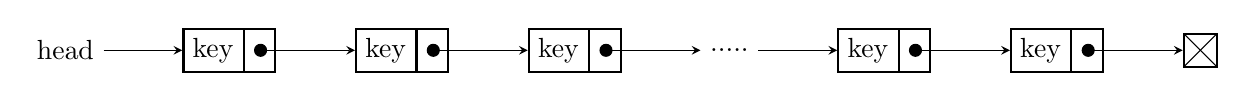
\begin{tikzpicture}
        [>=stealth, start chain]
        \node (a) {head};
        \begin{scope}[every node/.style=single-linked]
          \node[right=of {a}] (b) {key};
          \node[right=of {b}] (c) {key};
          \node[right=of {c}] (d) {key};
        \end{scope}

        \node[right=of {d}] (e) {.....};

        \begin{scope}[every node/.style=single-linked]
          \node[right=of {e}] (f) {key};
          \node[right=of {f}] (g) {key};
        \end{scope}

        \node[thick, on chain, draw,inner sep=6pt] (h) {};
        \draw[shorten <= 1pt, shorten >= 1pt] (h.north east) -- (h.south west);
        \draw[shorten <= 1pt, shorten >= 1pt] (h.north west) -- (h.south east);

        \draw[->] (a) -- (b);
        \draw[*->] let \p1=(b.two), \p2=(b.center) in (\x1,\y2) -- (c);
        \draw[*->] let \p1=(c.two), \p2=(c.center) in (\x1,\y2) -- (d);
        \draw[*->] let \p1=(d.two), \p2=(d.center) in (\x1,\y2) -- (e);
        \draw[->] (e) -- (f);
        \draw[*->] let \p1=(f.two), \p2=(d.center) in (\x1,\y2) -- (g);
        \draw[*->] let \p1=(g.two), \p2=(g.center) in (\x1,\y2) -- (h);
      \end{tikzpicture}
      \caption{Eigene Linked List-Klasse auf Basis der Vorlesung}
    \end{figure}

    \clearpagesolution

    \begin{subtask*}[credit=\stars{1}{3}]{Neues Element hinzufügen}
      Implementieren Sie die Methode \inlinejava{void add(T key)}. Diese bekommt einen neuen
      Schlüssel übergeben und erstellt ein neues Listenelement mit dem übergebenen Schlüssel,
      welches ganz am Ende der Liste angehängt wird.

      \br

      Denken Sie an den Spezialfall, wenn noch kein Element in der Liste vorhanden ist.

      \begin{solution}
        \lstinputlisting[style=Java]{codes/V1_1_Solution.java}
      \end{solution}
    \end{subtask*}

    \clearpagesolution

    \begin{subtask*}[credit=\stars{1}{3}]{Element entfernen I}
      Implementieren Sie die Methode \inlinejava{void delete}(int pos). Die Methode entfernt das
      Element an der Position \inlinejava{pos} aus der Liste, wobei das erste Element die
      Position \inlinejava{0} besitzt. Ist \inlinejava{pos} keine gültige Position, so wirft die
      Methode eine \inlinejava{IndexOutOfBoundsException} mit der Botschaft
      \code{\textcolor{stringcolor}{"'Invalid position!"'}}.

      \begin{solution}
        \lstinputlisting[style=Java]{codes/V1_2_Solution.java}
      \end{solution}
    \end{subtask*}

    \clearpagesolution

    \begin{subtask*}[credit=\stars{1}{3}]{Element entfernen II}
      Implementieren Sie die Methode \inlinejava{void delete(T key)}. Die Methode entfernt das
      erste wertgleiche Vorkommen des Elements \inlinejava{key} aus der Liste. Sollte das Element
      nicht vorkommen, so bleibt die Liste unverändert.

      \begin{solution}
        \lstinputlisting[style=Java]{codes/V1_3_Solution.java}
      \end{solution}
    \end{subtask*}

    \clearpagesolution

    \begin{subtask*}[credit=\stars{2}{3}]{Drittletztes Element}
      Implementieren Sie die Methode \inlinejava{T beforeBeforeLast()}. Der Rückgabewert der
      Methode ist \inlinejava{null}, falls die Liste nicht mindestens drei Elemente hat.
      Ansonsten wird der Key vom drittletzten Element der Liste zurückgeliefert.

      \begin{solution}
        \lstinputlisting[style=Java]{codes/V1_4_Solution.java}
      \end{solution}
    \end{subtask*}

    \clearpagesolution

    \begin{subtask*}[credit=\stars{2}{3}]{Eins nach links bitte}
      Implementieren Sie die Methode \inlinejava{void ringShiftLeft()}. Die Methode verschiebt
      alle Listenelemente um eine Stelle nach links. Das heißt, dass das erste Element das neue
      letzte Element der Liste wird.

      \begin{solution}
        \lstinputlisting[style=Java]{codes/V1_5_Solution.java}
      \end{solution}
    \end{subtask*}

    \clearpagesolution

    \begin{subtask*}[credit=\stars{2}{3}]{Liste in Array}
      Implementieren Sie (ohne einfach die zugehörige Methode aus der Standardbibliothek
      aufzurufen) die Methode \inlinejava{T[] listIntoArray(Class<?> type)}. Die Methode wandelt
      die Liste in ein Array um, das heißt genau alle Schlüsselwerte der Liste sind in dem Array,
      welches zurückgegeben wird, in ursprünglicher Reihenfolge enthalten. Sind keine
      Schlüsselwerte in der Liste enthalten, so soll ein Array der Länge null zurückgegeben werden.

      \begin{note}[title=Tipp:, color=tuda-orange]
        Ein Array des Typs \inlinejava{T} erstellen Sie am Besten auf folgende Weise:

        \begin{center}
          \href{https://docs.oracle.com/en/java/javase/11/docs/api/java.base/java/lang/reflect/Array.html#newInstance(java.lang.Class,int)}
          {\inlinejava{(T[]) Array.newInstance(type, size)}}
        \end{center}
      \end{note}

      \begin{solution}
        \lstinputlisting[style=Java]{codes/V1_6_Solution.java}
      \end{solution}
    \end{subtask*}

    \clearpagesolution

    \begin{subtask*}[credit=\stars{3}{3}]{Liste in Listen}
      \label{subtask:V1.7}
      Implementieren Sie die Methode \inlinejava{MyLinkedList<MyLinkedList<T>> listInLists()}.
      Die Methode teilt die Liste in eine Liste von mehreren einelementigen Listen auf, wobei
      jeder Schlüsselwert der Eingabeliste, zu genau einem Schlüsselwert einer einelementigen
      Liste wird.

      \begin{solution}
        \lstinputlisting[style=Java]{codes/V1_7_Solution.java}
      \end{solution}
    \end{subtask*}

    \clearpagesolution

    \begin{subtask*}[credit=\stars{3}{3}]{Quadratzahlen aus der Liste entfernen}
      Implementieren Sie die Methode \inlinejava{void} deleteSquareNumbers(). Die Methode
      entfernt alle Elemente aus der Liste, deren Position in der Liste eine Quadratzahl ist,
      wobei das erste Listenelement Position \inlinejava{0} hat.\footnote{0 ist natürlich auch
      eine Quadratzahl}

      \begin{solution}
        \lstinputlisting[style=Java]{codes/V1_8_Solution.java}
      \end{solution}
    \end{subtask*}

    \clearpagesolution

    \begin{subtask*}[credit=\stars{3}{3}]{Listen in Liste}
      Implementieren Sie die Methode
      \inlinejava{MyLinkedList<T> listsInList(MyLinkedList<MyLinkedList<T>> lsts)}.
      Die Methode erstellt eine zusammenhängende Liste aus dem Parameter \inlinejava{lsts}. Dazu
      sollen alle Listen des Parameters \inlinejava{lsts} in der ursprünglichen Reihenfolge
      hintereinander angefügt werden und die daraus resultierenden neue Liste zurückgegeben
      werden. Vergleichen Sie dazu auch nochmal Aufgabe
      \hyperref[subtask:V1.7]{V1.7}.

      \begin{solution}
        \lstinputlisting[style=Java]{codes/V1_9_Solution.java}
      \end{solution}
    \end{subtask*}
  \end{task}

  \clearpage

  \begin{task}[credit=\stars{3}{3}]{Eigene verzeigerte Struktur in Racket}
    In Racket haben Sie Listen schon einige Male gesehen und benutzt. In dieser Aufgabe wollen
    wir uns nach dem Vorbild von Aufgabe \hyperref[task:V1]{V1} eine eigene verzeigerte Struktur
    erstellen. Dafür ist bereits folgende Struktur vorgegeben:

    \lstinputlisting[style=Racket]{codes/V2_Task.rkt}

    Im Feld \inlineracket{value} des Structs wird der Schlüsselwert eines jeden
    \inlineracket{lst-item}s gespeichert. Im Feld \inlineracket{next}, wird der Nachfolger eines
    \inlineracket{lst-item}s gespeichert. Der Nachfolger ist entweder ebenfalls ein
    \inlineracket{lst-item} oder \inlinejava{null}, wenn es keinen Nachfolger gibt.

    \begin{subtask*}{Sortieren der Liste in aufsteigender Reihenfolge}
      Definieren Sie eine Funktion \inlineracket{sort-lst}.

      \br

      Diese bekommt den Kopf einer Liste übergeben, sortiert die \inlineracket{value}s der
      Elemente aufsteigend und liefert den Kopf dieser aufsteigend sortierten Liste zurück. Sie
      können davon ausgehen, dass die Liste nur Zahlen enthält. Benutzen Sie die Funktion
      \inlineracket{null?} um zu überprüfen, ob das letzte Element der Liste erreicht wurde. In
      diesem Fall gibt die Funktion \inlineracket{null?} dann \inlineracket{true} zurück, wenn
      damit das \inlineracket{next}-Feld, der \inlineracket{lst-item}-Struktur überprüft wird.

      \clearpagesolution

      \begin{solution}
        \lstinputlisting[style=Racket]{codes/V2_1_Solution.rkt}
      \end{solution}
    \end{subtask*}
  \end{task}

  \clearpage

  \begin{task}{Alternative LinkedList}
    In der Vorlesung haben Sie außerdem eine alternative \inlinejava{LinkedList} Implementierung
    kennengelernt. Diese zeichnet sich dadurch aus, dass anstelle eines Keys pro Item der Liste,
    ein Array von Keys mit einer vorher festgelegten Größe verwendet wird. Wir nennen diese Art
    von Listen in dieser Aufgabe \inlinejava{ArrayList}.

    \br

    Gegeben sei dafür folgende Klasse für Listenelemente:

    \lstinputlisting[style=Java]{codes/V3_01_Task.java}

    Alle nachfolgenden Aufgaben sollen dabei in folgender Klasse implementiert werden:

    \lstinputlisting[style=Java]{codes/V3_02_Task.java}

    \begin{figure}[h]
      \centering
      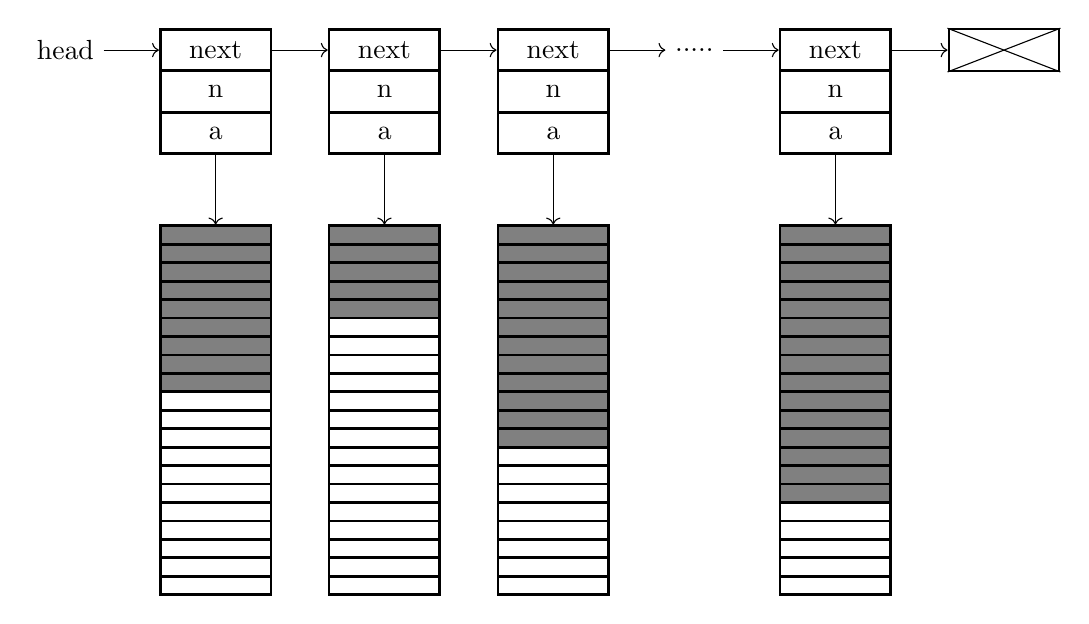
\begin{tikzpicture}
        \newcommand{\arraynext}[3]
        {
          \node[right=20pt of {#2}] (next#1) {next};
          \node[below=of {next#1}] (n#1) {n};
          \node[below=of {n#1}] (a#1) {a};
          \ifnum 0<#3
        \node[below=25pt of {a#1}, minimum height=5pt, fill=gray] (#10) {};
        \else
        \node[below=25pt of {a#1}, minimum height=5pt] (#10) {};
        \fi
        \foreach \i in {1, ..., 19}
            {
            \ifnum \i<#3
            \node[below=of {#1\the\numexpr\i-1\relax}, minimum height=5pt, fill=gray] (#1\i) {};
            \else
            \node[below=of {#1\the\numexpr\i-1\relax}, minimum height=5pt] (#1\i) {};
            \fi
          }

          \draw[->] (#2) -- (next#1);
        \draw[->] (a#1) -- (#10);
        }
        \node (head) {head};

        \begin{scope}[every node/.style=array-linked-item]
          \arraynext{1}{head}{9}
          \arraynext{2}{next1}{5}
          \arraynext{3}{next2}{12}
        \end{scope}

        \node[right=20pt of {next3}] (dots) { ..... };
        \draw[->] (next3) -- (dots);

        \begin{scope}[every node/.style=array-linked-item]
          \arraynext{4}{dots}{15}
          \node[right=20pt of {next4}, thick, draw,inner sep=6pt] (tail) {};
          \draw[->] (next4) -- (tail);
          \draw (tail.south west) -- (tail.north east)
          (tail.north west) -- (tail.south east);
        \end{scope}
      \end{tikzpicture}
      \caption{Eigene ArrayList-Klasse aus der Vorlesung}
    \end{figure}

    \begin{note}[title=Hinweis:, color=tuda-orange]
      Mit Index \(i\) bezeichnen wir den Schlüssel, welcher sich an Index \(i \mod n\) im Array
      des \(\lfloor i / n\rfloor\)-ten Listenelements befindet.
    \end{note}

    \begin{subtask*}[credit=\stars{1}{3}]{contains-Methode}
      Implementieren Sie die Methode \inlinejava{int contains(T e)}. Diese durchsucht die Liste
      nachdem übergebenen Element \inlinejava{e} und gibt den ersten gefundenen Index in der
      Liste zurück, sofern es dort enthalten ist. Ist das übergebene Element nicht enthalten,
      soll stattdessen \inlinejava{-1} zurückgegeben werden.

      \begin{solution}
        \lstinputlisting[style=Java]{codes/V3_1_Solution.java}
      \end{solution}
    \end{subtask*}

    \clearpagesolution

    \begin{subtask*}[credit=\stars{1}{3}]{get-Methode}
      Implementieren Sie die Methode \inlinejava{T get(int index)}. Diese gibt das Element an dem
      übergebenen Index in der Liste zurück. Eine \inlinejava{IndexOutOfBoundsException} soll
      geworfen werden, wenn der übergebene Index kleiner null ist oder der Index die Größe der
      Liste überschreitet.

      \begin{solution}
        \lstinputlisting[style=Java]{codes/V3_2_Solution.java}
      \end{solution}
    \end{subtask*}

    \clearpagesolution

    \begin{subtask*}[credit=\stars{2}{3}]{set-Methode}
      Implementieren Sie die Methode \inlinejava{void set(T e, int i)}. Diese bekommt ein
      Elemente vom Typ \inlinejava{T} und einen Index \inlinejava{i} übergeben und ersetzt das
      aktuelle Element am Index der Liste mit dem übergebenen. Eine
      \inlinejava{IndexOutOf-BoundsException} soll geworfen werden, wenn der übergebene Index
      kleiner null ist oder der Index die Größe der Liste überschreitet.

      \begin{solution}
        \lstinputlisting[style=Java]{codes/V3_3_Solution.java}
      \end{solution}
    \end{subtask*}

    \clearpagesolution

    \begin{subtask*}[credit=\stars{2}{3}]{remove-Methode}
      Implementieren Sie die Methode \inlinejava{void remove(int i)}. Diese bekommt einen Index
      \inlinejava{i} übergeben und entfernt das Element am übergebenen Index in der Liste. Alle
      nachfolgenden Elemente der Liste müssen daher um einen Index nach vorne verschoben werden,
      somit wird bei jedem nachfolgenden Element der Index dadurch um \inlinejava{1} geringer.
      War das zu entfernende Element das letzte Element in dem Array seines
      \inlinejava{ArrayListItem}s, so muss der Verweis auf dieses \inlinejava{ArrayListItem} auf
      \inlinejava{null} gesetzt werden, da es nicht mehr verwendet wird. Eine
      \inlinejava{IndexOutOfBoundsException} soll geworfen werden, wenn der übergebene Index
      kleiner \inlinejava{0} ist oder der Index die Größe der Liste überschreitet.

      \begin{solution}
        \lstinputlisting[style=Java]{codes/V3_4_Solution.java}
      \end{solution}
    \end{subtask*}

    \clearpagesolution

    \begin{subtask*}[credit=\stars{3}{3}]{Komprimierung}
      Implementieren sie die Methode \inlinejava{void compress()}, welche die Liste komprimiert.
      Das heißt, nach Aufruf der Methode müssen alle internen Arrays bis auf das Letzte komplett
      befüllt sein. Das letzte Array muss hierbei mindestens ein Element ungleich
      \inlinejava{null} enthalten, das heißt es muss \(n > 0\) gelten.

      \begin{figure}[h]
        \centering
        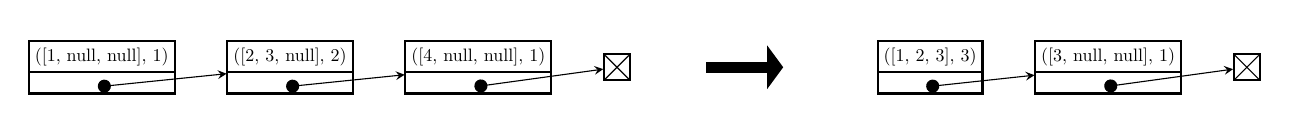
\begin{tikzpicture}
          [>=stealth, start chain, scale=.65, transform shape]
          \begin{scope}[every node/.style=array-linked]
            \node (a) {([1, \inlinejava{null}, \inlinejava{null}], 1)};
            \node[right=of a] (b) {([2, 3, \inlinejava{null}], 2)};
            \node[right=of b] (c) {([4, \inlinejava{null}, \inlinejava{null}], 1)};
          \end{scope}

          \node[
            thick,
            on chain,
            draw,
            inner sep=6pt,
            scale=1.2,
            transform shape,
            right=of c
          ] (d) {};
          \draw[shorten <= 1pt, shorten >= 1pt] (d.north east) -- (d.south west);
          \draw[shorten <= 1pt, shorten >= 1pt] (d.north west) -- (d.south east);

          \draw[*->] let \p1=(a.two), \p2=(a.two) in (\x1,\y2) -- (b);
          \draw[*->] let \p1=(b.two), \p2=(b.two) in (\x1,\y2) -- (c);
          \draw[*->] let \p1=(c.two), \p2=(c.two) in (\x1,\y2) -- (d);

          \node[scale=3, transform shape, right=of d] (arrow) {
            \arrow{.5}
          };

          \begin{scope}[every node/.style=array-linked]
            \node[right=of arrow](e) {([1, 2, 3], 3)};
            \node[right=of e] (f) {([3, \inlinejava{null}, \inlinejava{null}], 1)};
          \end{scope}

          \node[
            thick,
            on chain,
            draw,
            inner sep=6pt,
            scale=1.2,
            transform shape,
            right=of f
          ] (g) {};
          \draw[shorten <= 1pt, shorten >= 1pt] (g.north east) -- (g.south west);
          \draw[shorten <= 1pt, shorten >= 1pt] (g.north west) -- (g.south east);

          \draw[*->] let \p1=(e.two), \p2=(e.two) in (\x1,\y2) -- (f);
          \draw[*->] let \p1=(f.two), \p2=(f.two) in (\x1,\y2) -- (g);
        \end{tikzpicture}
        \caption{Beispiel für \inlinejava{compress()} mit \(N=3\)}
      \end{figure}

      \begin{solution}
        \lstinputlisting[style=Java]{codes/V3_5_Solution.java}
      \end{solution}
    \end{subtask*}
  \end{task}
\end{document}
